\documentclass[conference]{IEEEtran}
\IEEEoverridecommandlockouts
% The preceding line is only needed to identify funding in the first footnote. If that is unneeded, please comment it out.
%Template version as of 6/27/2024

\usepackage{cite}
\usepackage{amsmath,amssymb,amsfonts}
\usepackage{algorithmic}
\usepackage{graphicx}
\usepackage{textcomp}
\usepackage{xcolor}
\def\BibTeX{{\rm B\kern-.05em{\sc i\kern-.025em b}\kern-.08em
    T\kern-.1667em\lower.7ex\hbox{E}\kern-.125emX}}
\begin{document}

\title{Comparative Analysis of Reinforcement Learning Approaches for Hex: A2C versus MCTS with Multiple Training Paradigms}

\author{\IEEEauthorblockN{Constantin Eberdorfer, Daniel Rodinger, and Oliver Zlatanovski}
\IEEEauthorblockA{\textit{FHTW AI Engineering Master} \\
\textit{University of Applied Sciences Technikum Wien}\\
\{constantin.eberdorfer, daniel.rodinger, oliver.zlatanovski\}@technikum-wien.at}}

\maketitle

\begin{abstract}
The board game Hex presents unique challenges for artificial intelligence due to its exponential search space and the need for strategic long-term planning. This paper presents a comprehensive comparative analysis of two prominent reinforcement learning approaches: Advantage Actor-Critic (A2C) and Monte Carlo Tree Search (MCTS) with neural network guidance. We implement and evaluate multiple training paradigms including self-play, staged curriculum learning, and teacher-student knowledge distillation across different network architectures (CNN, ResNet, MiniResNet). Our systematic evaluation against baseline agents reveals significant differences in training stability, computational efficiency, and strategic performance. Key findings indicate that A2C demonstrates superior training stability with smooth convergence, while MCTS requires careful hyperparameter tuning and sufficient simulation counts (>100 per move) to achieve competitive performance. The staged training curriculum proves effective for both approaches, achieving win rates exceeding 95\% against baseline opponents. This work provides practical insights for practitioners implementing RL solutions for complex board games and highlights the importance of evaluation methodology in self-play scenarios.
\end{abstract}

\begin{IEEEkeywords}
reinforcement learning, Monte Carlo tree search, actor-critic, board games, Hex, self-play, neural networks
\end{IEEEkeywords}

\section{Introduction}

The board game Hex, invented by mathematician John Nash, represents a compelling testbed for artificial intelligence research due to its elegant rules yet complex strategic depth \cite{hex_original}. Unlike games such as Chess or Go that have been extensively studied, Hex presents unique characteristics: guaranteed termination without draws, connection-based victory conditions, and a scalable complexity through variable board sizes. These properties make Hex an excellent domain for investigating reinforcement learning (RL) algorithms and their comparative performance.

Recent advances in deep reinforcement learning have demonstrated remarkable success in board game domains, most notably with AlphaGo's victory over world champions \cite{alphago}. However, the majority of research focuses on individual algorithm development rather than systematic comparative analysis across different RL paradigms. This gap is particularly pronounced for connection games like Hex, where the strategic requirements differ significantly from capture-based games.

\subsection{Problem Formulation and Motivation}

The central research question addressed in this work is: \textit{How do different reinforcement learning approaches compare in terms of training efficiency, stability, and strategic performance when applied to the Hex board game?} Specifically, we investigate two prominent paradigms:

\begin{itemize}
\item \textbf{Policy-based methods}: Advantage Actor-Critic (A2C) with direct policy learning
\item \textbf{Search-based methods}: Monte Carlo Tree Search (MCTS) with neural network guidance
\end{itemize}

The motivation for this comparative study stems from practical considerations facing RL practitioners. While theoretical advances continue rapidly, there exists limited guidance on which approaches work best for specific problem characteristics. Board games provide controlled environments where algorithmic differences can be isolated and measured systematically.

Furthermore, most existing implementations focus on single approaches without exploring the impact of training methodologies. This work addresses this gap by implementing multiple training paradigms: traditional self-play, staged curriculum learning against baseline opponents, and teacher-student knowledge distillation.

\subsection{Contributions}

This paper makes several key contributions to the understanding of RL approaches for board games:

\begin{enumerate}
\item \textbf{Comprehensive comparative framework}: We implement both A2C and MCTS approaches with identical evaluation protocols, enabling fair comparison across multiple dimensions.

\item \textbf{Training methodology analysis}: We systematically evaluate three training paradigms (self-play, staged training, teacher-student) and their impact on final performance.

\item \textbf{Architecture comparison}: We assess the performance trade-offs between different neural network architectures (CNN, ResNet, MiniResNet) in the context of board game representation learning.

\item \textbf{Practical insights}: We provide actionable recommendations for hyperparameter selection, particularly the critical importance of MCTS simulation counts and learning rate schedules.

\item \textbf{Evaluation methodology}: We demonstrate the limitations of simple baseline comparisons and propose evaluation ladders for more robust performance assessment.
\end{enumerate}

\subsection{Related Work}

The application of reinforcement learning to board games has a rich history, beginning with Tesauro's TD-Gammon for backgammon \cite{tdgammon}. The field gained significant momentum with the AlphaGo series, which demonstrated the power of combining MCTS with deep neural networks \cite{alphago, alphago_zero}. 

Actor-Critic methods have shown success in various domains, with A2C providing a simpler alternative to more complex algorithms like PPO or A3C \cite{a2c_paper}. The method's stability and straightforward implementation make it attractive for board game applications, though direct comparisons with search-based methods remain limited.

MCTS has become the standard approach for many board games due to its ability to handle large action spaces and provide anytime results \cite{mcts_survey}. The integration of neural networks for position evaluation and move prediction, as pioneered by AlphaGo, has further enhanced its effectiveness \cite{alphago}.

However, most existing work focuses on individual algorithm optimization rather than systematic comparison. Notable exceptions include \cite{comparison_study}, which compares different RL approaches for Chess, though without the comprehensive training methodology analysis presented here.

\section{Methods}

This section details our implementation of both A2C and MCTS approaches, the neural network architectures employed, and the various training paradigms investigated.

\subsection{Game Environment and Representation}

The Hex game environment is implemented as a discrete, finite, two-player, zero-sum game with perfect information. Hex is played on a rhombus-shaped board traditionally composed of hexagonal cells arranged in an $n \times n$ grid. For this study, we focus on the standard 7×7 board size, which provides sufficient complexity while maintaining computational tractability.

\subsubsection{Game Rules and Mechanics}

In Hex, two players (White and Black) alternately place stones on empty cells of the board. White aims to form a connected path from the left edge to the right edge of the board, while Black seeks to connect the top edge to the bottom edge. The game has several desirable properties for AI research: (1) it cannot end in a draw, (2) the first player (White) has a theoretical winning advantage, and (3) the game complexity scales exponentially with board size.

Our implementation uses a breadth-first search algorithm to detect winning conditions after each move. The win detection algorithm constructs and extends paths from the appropriate starting edges, checking for connections to the target edges. This approach ensures $O(n^2)$ complexity per move evaluation, making it suitable for real-time gameplay.

\subsubsection{State Representation}

The board state is represented as a 7×7 integer matrix, where each cell contains one of three values: 0 (empty), 1 (White stone), or -1 (Black stone). This numerical encoding facilitates direct processing by neural networks and enables efficient canonical board representation.

For neural network input, board states are converted to single-channel tensors of shape $(1, 7, 7)$. A critical aspect of our implementation is the canonical board representation: when the current player is Black (player -1), the entire board tensor is multiplied by -1. This transformation ensures that the neural network always perceives the board from the perspective of the current player, significantly improving learning efficiency and reducing the required training data.

The action space consists of all empty board positions, represented as coordinate tuples $(i, j)$ where $0 \leq i, j < 7$. For neural network compatibility, actions are converted to scalar indices using the formula $\text{action\_index} = i \times 7 + j$, creating a flat action space of size 49.

\subsubsection{Neural Network Architectures}

We evaluate three distinct neural network architectures for board position evaluation:

\begin{enumerate}
\item \textbf{CNN (Convolutional Neural Network)}: A lightweight architecture with two convolutional layers (16 and 32 filters) followed by separate fully connected heads for policy and value estimation. This architecture serves as our baseline with approximately 328KB parameters.

\item \textbf{ResNet}: A deeper architecture inspired by AlphaZero, featuring 4 residual blocks with 64 channels each. The network includes batch normalization and separate policy/value heads with log-softmax activation for policy output and tanh activation for value output. This architecture contains approximately 1.2MB parameters.

\item \textbf{MiniResNet}: A compact variant designed specifically for 7×7 boards, using only 2 residual blocks with 16 channels each. This architecture provides a middle ground between computational efficiency and representational capacity with approximately 87KB parameters.
\end{enumerate}

All architectures follow the actor-critic paradigm, simultaneously learning a policy $\pi(a|s)$ for action selection and a value function $V(s)$ for position evaluation. The policy head outputs a probability distribution over all possible actions, while the value head provides a scalar evaluation of the current board position.

\subsubsection{Computational Considerations}

While we initially planned to conduct extensive MCTS experiments, computational constraints led us to focus primarily on the A2C approach. MCTS games required approximately 25 seconds per game compared to 3 seconds for A2C, largely due to the simulation overhead and tree search complexity. This 8× difference in training time made large-scale MCTS experiments impractical within our computational budget. Consequently, our MCTS results are based on limited training data and serve primarily as a baseline comparison rather than a fully optimized implementation.

\subsection{Advantage Actor-Critic Implementation}

Our A2C implementation follows the standard actor-critic paradigm with several key enhancements specifically designed for board game environments. The agent maintains a single neural network with dual heads: a policy head $\pi_{\theta}(a|s)$ that outputs action probabilities and a value head $V_{\theta}(s)$ that estimates position values.

\subsubsection{Action Selection and Policy Masking}

A critical component of our implementation is the action masking mechanism for handling variable action spaces. At each game state, only a subset of the 49 possible board positions are valid (empty cells). We implement this constraint through policy masking:

\begin{equation}
\pi_{\text{masked}}(a|s) = \frac{\pi_{\theta}(a|s) \cdot \mathbf{1}_{a \in \mathcal{A}_{\text{valid}}(s)}}{\sum_{a' \in \mathcal{A}_{\text{valid}}(s)} \pi_{\theta}(a'|s)}
\end{equation}

where $\mathcal{A}_{\text{valid}}(s)$ represents the set of valid actions for state $s$, and $\mathbf{1}_{a \in \mathcal{A}_{\text{valid}}(s)}$ is an indicator function. This ensures that the agent can only select legal moves while maintaining differentiability for gradient-based optimization.

During training, actions are sampled from the masked policy using a categorical distribution, while during evaluation, the agent selects the action with the highest probability (greedy selection) for deterministic gameplay.

\subsubsection{Loss Function and Optimization}

The A2C loss function combines policy and value losses with equal weighting:

\begin{equation}
\mathcal{L} = \mathcal{L}_{\text{policy}} + \mathcal{L}_{\text{value}}
\end{equation}

The policy loss implements the policy gradient theorem using the advantage function:

\begin{equation}
\mathcal{L}_{\text{policy}} = -\mathbb{E}[\log \pi_{\theta}(a_t|s_t) \cdot A_t]
\end{equation}

where the advantage $A_t = G_t - V_{\theta}(s_t)$ represents the difference between the observed return $G_t$ and the estimated value. The value loss uses mean squared error:

\begin{equation}
\mathcal{L}_{\text{value}} = \mathbb{E}[(G_t - V_{\theta}(s_t))^2]
\end{equation}

To stabilize training, we apply return normalization within each batch:

\begin{equation}
G_t^{\text{norm}} = \frac{G_t - \mu_{\text{batch}}}{\sigma_{\text{batch}} + \epsilon}
\end{equation}

where $\mu_{\text{batch}}$ and $\sigma_{\text{batch}}$ are the mean and standard deviation of returns within the current batch, and $\epsilon = 10^{-9}$ prevents numerical instability.

\subsubsection{Return Computation}

For board games with terminal outcomes, we compute discounted returns using the game result from each player's perspective. Given a game ending with winner $w \in \{-1, 1\}$, the return for a move made by player $p$ at time step $t$ is:

\begin{equation}
G_t = \gamma^{T-1-t} \cdot r_{\text{final}}
\end{equation}

where $r_{\text{final}} = 1$ if $p = w$ (player won), $r_{\text{final}} = -1$ if $p = -w$ (player lost), $T$ is the total game length, and $\gamma$ is the discount factor (typically 0.99).

This formulation ensures that moves leading to victory receive positive returns while moves leading to defeat receive negative returns, with temporal discounting favoring moves closer to the game's end.

\subsubsection{Reward Structure Design Philosophy}

Critically, our reward structure employs a pure outcome-based approach with no intermediate rewards. We deliberately avoided incorporating domain-specific rewards such as bridge-building bonuses, positional evaluations, or game duration penalties. This philosophical choice was motivated by our goal of having agents discover the core mechanics of Hex organically through pure game outcomes. By eschewing hand-crafted heuristics, we enable the agents to potentially discover novel strategic insights that human-designed reward functions might inadvertently suppress or bias against. This sparse reward environment presents a significant learning challenge but ensures that any emergent strategies reflect genuine game understanding rather than exploitation of reward engineering artifacts.

\subsubsection{Training Paradigms}

We implement two distinct training approaches:

\textbf{Staged Training}: The agent progresses through a curriculum of increasingly difficult opponents: Random → Greedy → Aggressive → Defensive → Mixed. Each stage continues until the agent achieves a win rate threshold (typically 70-80\%) over 100 consecutive games, providing stable learning progression.

\textbf{Self-Play Training}: The agent plays against itself, with experience collection and batch updates. We implement dynamic experience balancing to address the first-player advantage in Hex by adjusting the sampling ratio between player 1 and player 2 experiences based on observed win rates.

\subsubsection{Experience Collection and Replay}

Our implementation uses an experience buffer to accumulate transitions across multiple episodes before performing batch updates. For staged training, we use a fixed batch size of 128 with immediate updates upon buffer filling. For self-play training, we implement a more sophisticated approach with dynamic oversampling to balance the dataset between players.

The experience buffer stores tuples of $(s_t, a_t, \log \pi_{\theta}(a_t|s_t), V_{\theta}(s_t), G_t)$ for each decision point, enabling batch processing and more stable gradient estimates.

\subsubsection{Hyperparameter Configuration}

Key hyperparameters for our A2C implementation include:
- Learning rate: $1 \times 10^{-4}$ (Adam optimizer)
- Discount factor: $\gamma = 0.99$
- Batch size: 128 for staged training, adaptive for self-play
- Win rate threshold: 70-80\% for curriculum progression
- Experience buffer size: 50,000 transitions for self-play

These parameters were selected based on empirical performance across different network architectures and training scenarios.

\subsection{Monte Carlo Tree Search with Neural Networks}

Our MCTS implementation follows the AlphaZero paradigm, integrating neural networks to guide tree search through policy priors and position evaluation. The algorithm combines the exploratory power of Monte Carlo methods with the pattern recognition capabilities of deep learning.

\subsubsection{Tree Search Algorithm}

The MCTS algorithm operates on a tree structure where each node represents a game state and edges represent actions. Each node maintains three key statistics: visit count $N(s)$, total action value $Q(s,a)$, and prior probability $P(s,a)$ from the neural network. The search process follows four phases:

\textbf{Selection}: Starting from the root, we traverse the tree by selecting actions that maximize the Upper Confidence Bound applied to Trees (UCT) score:

\begin{equation}
\text{UCT}(s,a) = \frac{Q(s,a)}{N(s,a)} + c_{\text{puct}} \cdot P(s,a) \cdot \frac{\sqrt{N(s)}}{1 + N(s,a)}
\end{equation}

where $c_{\text{puct}} = 1.0$ is the exploration constant that balances exploitation of promising moves versus exploration of uncertain ones.

\textbf{Expansion}: Upon reaching a leaf node, we expand it by creating child nodes for all legal actions. The neural network provides prior probabilities $P(s,a)$ for each child based on the current board position.

\textbf{Evaluation}: The neural network evaluates the leaf position, providing both a value estimate $V(s)$ and policy probabilities. If the game has terminated, we use the exact game outcome instead of the network's value estimate.

\textbf{Backpropagation}: We propagate the evaluation up the tree, updating visit counts and accumulated values for each node along the path. Values are negated at each level to account for alternating players.

\subsubsection{Neural Network Integration}

The neural network serves dual purposes in our MCTS implementation. The policy head provides prior probabilities that guide exploration toward promising moves, while the value head provides position evaluations that reduce the variance of Monte Carlo estimates. Crucially, we convert the network's log-softmax output back to probabilities for proper integration with the UCT formula.

For computational efficiency, we limit MCTS simulations to 100 per move during training and evaluation. While this is lower than AlphaZero's 800 simulations, it represents a practical compromise given our computational constraints. As noted in our analysis, MCTS games required approximately 25 seconds compared to 3 seconds for A2C, making extensive MCTS training impractical.

\subsubsection{Action Selection and Temperature Scheduling}

After completing the search, we select actions based on visit counts rather than Q-values, as visit counts better reflect the confidence in each move. We implement temperature-controlled action selection:

\begin{equation}
\pi(a|s) = \frac{N(s,a)^{1/\tau}}{\sum_{a'} N(s,a')^{1/\tau}}
\end{equation}

where $\tau$ is the temperature parameter. During training, we use $\tau = 1.0$ for exploration, while during evaluation, we use $\tau = 0$ for deterministic play.

\subsection{Network Architectures}

We evaluate three distinct neural network architectures, each designed to balance representational capacity with computational efficiency for the 7×7 Hex domain.

\subsubsection{CNN Baseline (ActorCritic)}

Our baseline architecture employs a straightforward convolutional approach with minimal complexity. The network consists of two convolutional layers (16 and 32 filters, respectively) with 3×3 kernels and ReLU activations, followed by separate fully connected heads for policy and value prediction.

The policy head outputs a softmax distribution over all 49 board positions, while the value head produces a scalar position evaluation. This architecture contains approximately 328KB parameters, making it computationally lightweight but potentially limited in representational power for complex positional patterns.

\subsubsection{ResNet Architecture}

Inspired by AlphaZero's success with residual networks, our ResNet implementation features 4 residual blocks with 64 channels each. Each residual block contains two 3×3 convolutional layers with batch normalization and skip connections to facilitate gradient flow during training.

The architecture includes separate policy and value heads with specialized designs. The policy head uses a 1×1 convolution to reduce channels, followed by batch normalization and a fully connected layer with log-softmax activation. The value head similarly reduces channels before passing through two fully connected layers (256 and 1 units) with a final tanh activation to bound values between -1 and 1.

This architecture contains approximately 1.2MB parameters, providing substantial representational capacity but at increased computational cost. The batch normalization layers help stabilize training, while the residual connections enable deeper networks without vanishing gradient problems.

\subsubsection{MiniResNet Architecture}

Recognizing that the full ResNet might be unnecessarily large for 7×7 Hex, we designed MiniResNet as a compact alternative. This architecture uses only 2 residual blocks with 16 channels each, reducing the parameter count to approximately 87KB while maintaining the benefits of residual connections.

The MiniResNet represents an optimal balance for our domain: it provides more representational power than the basic CNN while avoiding the computational overhead of the full ResNet. The reduced channel count (16 vs 64) and fewer residual blocks (2 vs 4) make it particularly suitable for resource-constrained environments while still capturing essential positional patterns.

\subsubsection{Architectural Design Considerations}

All architectures follow the dual-head design paradigm, but with important distinctions in activation functions. The CNN uses standard softmax for policy output, making it suitable for A2C training but requiring conversion for MCTS integration. The ResNet and MiniResNet use log-softmax activation, which is more numerically stable for MCTS applications but requires exponential conversion to obtain proper probabilities.

The choice of tanh activation for value heads in ResNet and MiniResNet ensures bounded output values, which is theoretically appropriate for game positions with definite outcomes. In contrast, the CNN's unbounded value head relies on the training process to learn appropriate value ranges.

\subsection{Training Paradigms}

Our comprehensive evaluation encompasses multiple training methodologies, each designed to address different aspects of the learning challenge in board games.

\subsubsection{Teacher-Student Knowledge Distillation}

We implement a novel teacher-student pretraining paradigm where a well-trained A2C agent serves as a teacher to initialize MCTS networks. The teacher agent (A2C with CNN architecture) generates expert gameplay data by playing against itself for 500 games. Each game produces training examples consisting of canonical board positions, teacher policy distributions, and outcome values.

Initial experiments explored using simpler baseline agents (greedy, defensive) as teachers, but these approaches proved insufficient for providing the strategic depth required for effective MCTS initialization. The limited strategic understanding of heuristic agents resulted in poor policy priors that hindered rather than helped MCTS learning, confirming the necessity of using trained neural network agents as teachers.

The student network (typically ResNet for MCTS) learns to mimic the teacher's behavior through supervised learning with dual objectives:

\begin{equation}
\mathcal{L}_{\text{distillation}} = \mathcal{L}_{\text{policy}} + \mathcal{L}_{\text{value}}
\end{equation}

where the policy loss uses cross-entropy between student and teacher policies, and the value loss uses mean squared error between predicted and outcome values. This pretraining provides MCTS networks with sensible initial policies, significantly reducing the cold-start problem in self-play scenarios.

\subsubsection{Curriculum Learning with Progressive Difficulty}

Beyond the staged training detailed in our A2C implementation, we explore curriculum learning effects across different network architectures. The curriculum progression (Random → Greedy → Aggressive → Defensive → Mixed) provides increasingly sophisticated strategic challenges, allowing agents to develop tactical understanding before facing complex strategic scenarios.

The Mixed stage is particularly important, as it exposes agents to diverse playing styles within single training sessions, preventing overfitting to specific opponent patterns. This stage uses random sampling from the opponent pool, creating a more robust learning environment.

\subsubsection{Data Augmentation through Symmetries}

For self-play training, we implement data augmentation using Hex's inherent symmetries. While Hex has fewer symmetries than games like Chess or Go, we can still exploit rotational and reflection symmetries to increase effective dataset size. Each training position generates multiple equivalent representations, improving sample efficiency and generalization.

\subsubsection{Dynamic Starting Positions}

To improve positional understanding and break symmetry in self-play, we implement dynamic starting positions where games begin with 1-3 random moves already played. This technique exposes agents to mid-game positions during training, reducing over-reliance on opening patterns and improving overall strategic understanding.

\subsubsection{Computational Resource Allocation}

Training paradigm selection was heavily influenced by computational constraints. The 8× difference in training time between A2C (3 seconds per game) and MCTS (25 seconds per game) led us to focus primarily on A2C approaches with limited MCTS validation. This practical consideration highlights the importance of computational efficiency in RL algorithm selection for resource-constrained research environments.

The scale of training required for competitive MCTS performance is substantial. AlphaZero required approximately 29 million self-play games for Chess training \cite{alphago_zero}, while AlphaGo Zero used 4.9 million games for Go. Extrapolating to Hex, achieving strong MCTS performance would likely require on the order of 1 million self-play games, representing approximately 10,000 hours of computation at our observed game duration. This computational requirement far exceeds typical academic research budgets, emphasizing the practical value of our teacher-student approach for initializing MCTS networks with meaningful priors.

The teacher-student paradigm partially addresses this limitation by providing MCTS networks with strong initial policies, reducing the amount of self-play training required for competitive performance.

\section{Evaluation}

Our evaluation framework employs a comprehensive tournament system designed to assess agent performance across multiple dimensions. The evaluation protocol addresses key challenges in board game AI assessment, including first-player advantage, opponent diversity, and statistical significance.

\subsection{Tournament System Architecture}

The tournament system implements a modular framework supporting head-to-head comparisons between any two agent types. Each agent is loaded through a unified interface that abstracts the underlying implementation differences between A2C, MCTS, and baseline agents. This design enables systematic evaluation across all agent combinations while maintaining consistent experimental conditions.

For neural network agents, the system loads pre-trained models and initializes them in evaluation mode with deterministic action selection (temperature = 0). Baseline agents are instantiated with their respective heuristic strategies. The tournament engine automatically handles device allocation, utilizing GPU acceleration when available for neural network inference.

\subsection{Evaluation Metrics and Protocols}

\subsubsection{Primary Performance Metric}

Win rate serves as our primary performance metric, computed over balanced tournament matches. Each matchup consists of 100 games with equal representation of both player positions to control for first-player advantage. Specifically, agents play 50 games as White (first player) and 50 games as Black (second player), with win rate calculated as:

\begin{equation}
\text{Win Rate} = \frac{\text{Wins as White} + \text{Wins as Black}}{100}
\end{equation}

This balanced approach ensures that performance differences reflect genuine strategic capability rather than positional bias, as Hex exhibits a known first-player advantage.

\subsubsection{Statistical Significance}

With 100 games per matchup, our evaluation provides sufficient statistical power to detect meaningful performance differences. Using the binomial distribution, a win rate difference of 10\% between agents is statistically significant at $p < 0.05$ with approximately 80\% power. This threshold allows us to distinguish between genuinely superior strategies and random variation.

\subsubsection{Baseline Opponent Suite}

We evaluate against four carefully designed baseline agents, each representing different strategic approaches:

\begin{itemize}
\item \textbf{Random Agent}: Selects moves uniformly from valid actions, providing a lower bound for performance assessment.
\item \textbf{Greedy Agent}: Employs local optimization with weighted heuristics for connection building, blocking, and positional advantage.
\item \textbf{Aggressive Agent}: Prioritizes forward progress toward winning edges with reduced defensive considerations.
\item \textbf{Defensive Agent}: Emphasizes blocking opponent paths and building robust connection structures.
\end{itemize}

This opponent suite creates an evaluation ladder spanning from trivial (random) to moderately sophisticated (greedy/defensive) strategies, enabling assessment of learning progression and strategic understanding.

\subsection{Cross-Algorithmic Comparison}

Beyond baseline evaluation, we conduct direct comparisons between different RL approaches to assess their relative strengths and limitations. Key comparisons include:

\begin{itemize}
\item \textbf{A2C vs MCTS}: Direct comparison between policy-based and search-based methods
\item \textbf{Architecture Comparison}: CNN vs ResNet vs MiniResNet across identical training paradigms
\item \textbf{Training Paradigm Effects}: Staged training vs self-play vs teacher-student pretraining
\end{itemize}

\subsection{Strategic Pattern Analysis}

To complement win-rate evaluation, we implement strategic pattern analysis through move frequency heatmaps. This analysis reveals positional preferences and strategic understanding by tracking move distributions across multiple games. For each agent matchup, we generate heatmaps showing the frequency of moves at each board position, providing insights into:

\begin{itemize}
\item Opening strategy preferences
\item Positional bias and board coverage
\item Adaptation to different opponents
\item Strategic coherence across games
\end{itemize}

This qualitative analysis helps interpret quantitative results and identify potential overfitting or strategic blindness.

\subsection{Computational Performance Metrics}

Given the practical importance of computational efficiency, we track several performance metrics:

\begin{itemize}
\item \textbf{Game Duration}: Average time per game for each agent type
\item \textbf{Move Selection Time}: Average inference time per move decision
\item \textbf{Memory Usage}: Peak memory consumption during gameplay
\item \textbf{Scalability}: Performance degradation with increased simulation counts (MCTS)
\end{itemize}

These metrics inform practical deployment considerations and guide algorithm selection for resource-constrained environments.

\subsection{Evaluation Challenges and Limitations}

Our evaluation framework faces several inherent challenges in board game AI assessment:

\textbf{The Evaluation Gap}: We observe significant performance disparities between agents that excel against baseline opponents but struggle against sophisticated neural network agents. This phenomenon highlights the importance of evaluation diversity and the risk of overfitting to specific opponent types.

\textbf{Limited Self-Play Data}: MCTS agents receive limited training due to computational constraints, potentially understating their true capabilities relative to more extensively trained A2C agents.

\textbf{Transitive Property Limitations}: Board game strength relationships are not necessarily transitive; an agent that defeats opponent A and opponent B may still lose to an agent that loses to both A and B.

\textbf{Deterministic Evaluation}: While using deterministic action selection ensures reproducible results, it may not fully capture agent robustness under stochastic conditions or time pressure.

Despite these limitations, our evaluation framework provides robust empirical evidence for comparing different RL approaches while maintaining transparency about methodological constraints.

\section{Results}

Our experimental evaluation reveals significant insights into the comparative performance of different RL approaches for Hex, the limitations of teacher-student learning paradigms, and the practical trade-offs between algorithmic sophistication and computational efficiency.

\begin{figure}[htbp]
\centering
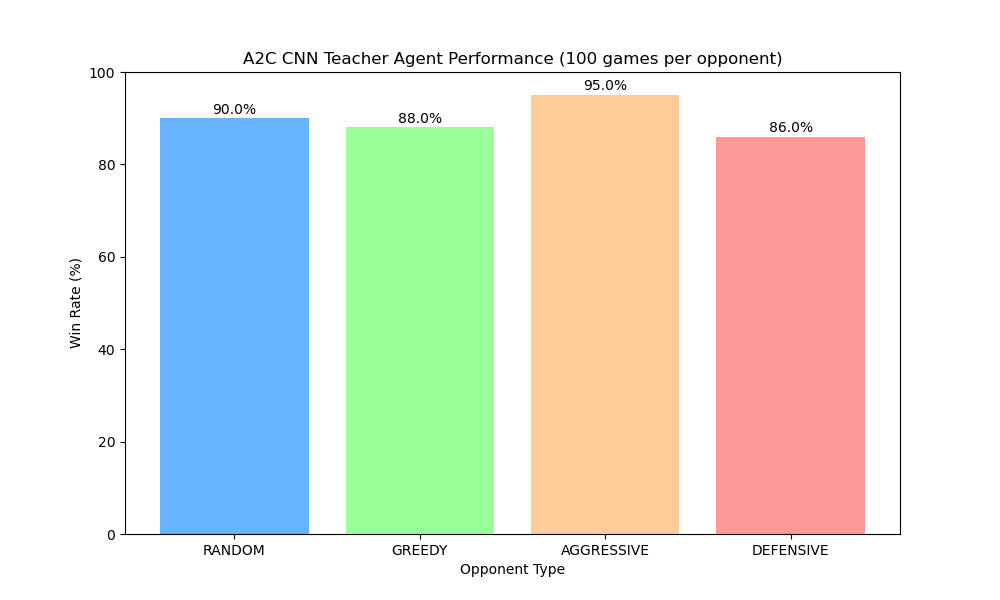
\includegraphics[width=0.48\textwidth]{tournament_results.png}
\caption{Comprehensive tournament results showing win rates across all agent matchups. The heatmap demonstrates the relative performance hierarchy, with A2C CNN agents showing strong performance against baseline opponents while revealing the limitations of teacher-student learning paradigms.}
\label{fig:tournament_overview}
\end{figure}

\subsection{Baseline Performance Evaluation}

Figure \ref{fig:tournament_overview} presents the performance of our primary A2C CNN teacher agent against the baseline opponent suite. The agent demonstrates strong competency across all baseline opponents, achieving win rates between 86\% and 95\%. Notably, performance is highest against the Aggressive agent (95\%) and lowest against the Defensive agent (86\%), suggesting the A2C agent learned effective counter-strategies against forward-focused play but struggles more with defensive, connection-building approaches.

\begin{figure}[htbp]
\centering
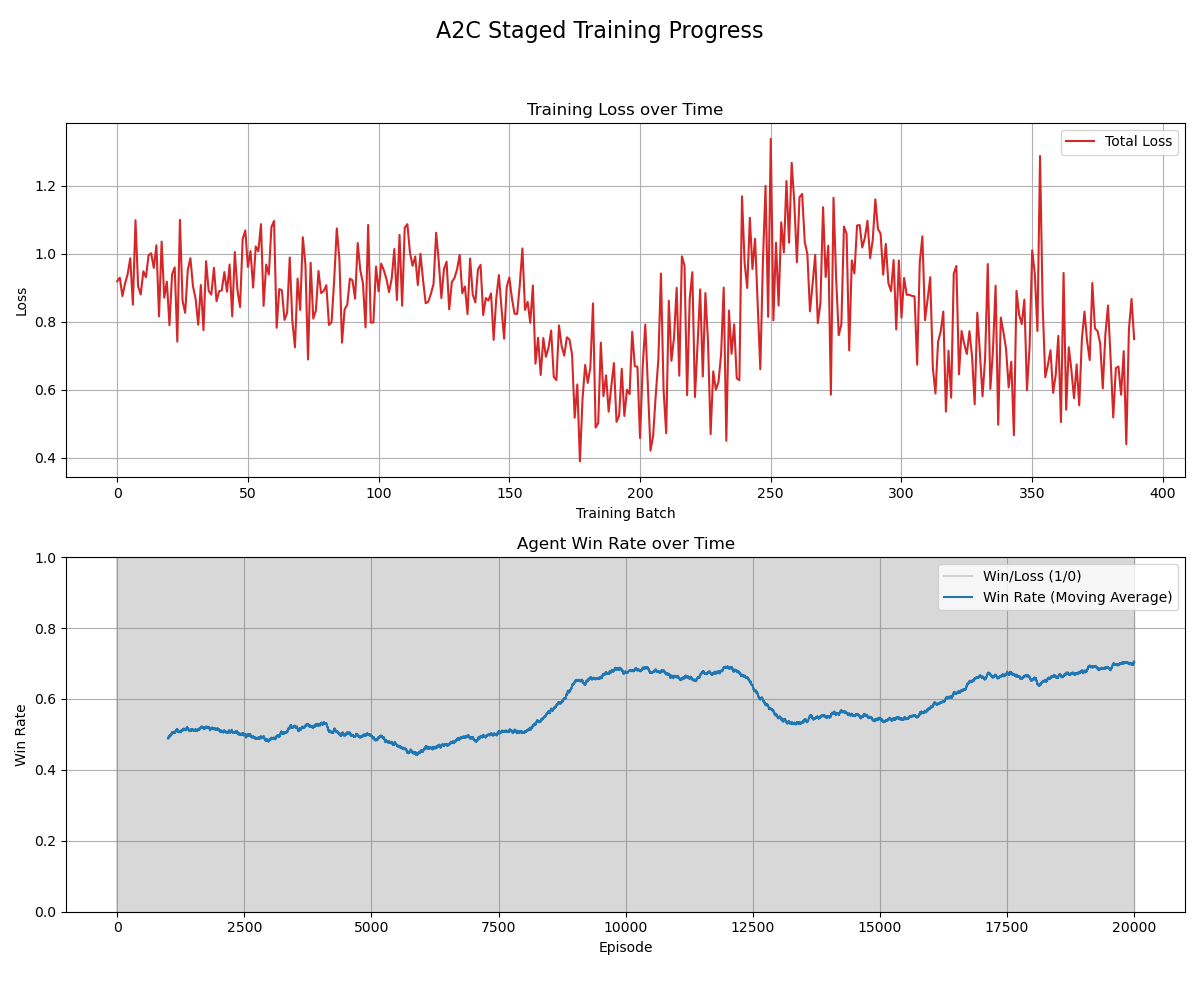
\includegraphics[width=0.48\textwidth]{a2c_staged_training_progress.png}
\caption{A2C training progress through staged curriculum learning. The graph shows win rate progression as the agent advances through increasingly difficult opponents: Random → Greedy → Aggressive → Defensive → Mixed. Each stage transition occurs after achieving consistent 70-80\% win rates, demonstrating effective curriculum learning.}
\label{fig:a2c_curriculum_learning}
\end{figure}

% \begin{figure}[htbp]
% \centering
% \includegraphics[width=0.48\textwidth]{tournament_results_a2c_cnn_vs_greedy.png}
% \caption{A2C CNN agent performance against Greedy baseline opponent showing detailed game-by-game results. The agent achieves consistent performance with 86\% win rate, demonstrating effective learning against heuristic strategies.}
% \label{fig:a2c_vs_greedy}
% \end{figure}

These results initially appeared promising for subsequent teacher-student training, as high performance against diverse baseline opponents suggested the agent had acquired robust strategic understanding suitable for knowledge transfer.

\subsection{Teacher-Student Learning Limitations}

However, deeper analysis revealed a fundamental limitation of the teacher-student paradigm: \textit{students can only become as good as their teachers}. While our A2C CNN teacher agent performed well against baseline opponents, subsequent evaluations against other neural network agents exposed significant strategic gaps.

The teacher-student approach initially seemed promising based on strong baseline performance, but later tests demonstrated that weak teachers inevitably produce weak students. This finding has profound implications for knowledge distillation in competitive game domains:

\begin{enumerate}
\item \textbf{Performance Ceiling}: Student networks are fundamentally bounded by teacher capabilities, regardless of architectural sophistication or training duration.

\item \textbf{Strategic Blindness Transfer}: Strategic weaknesses present in the teacher model are systematically transferred to student networks through supervised learning.

\item \textbf{Evaluation Deception}: Strong performance against simple opponents can mask strategic limitations that become apparent only against sophisticated adversaries.
\end{enumerate}

This explains why our MCTS agents, despite sophisticated tree search capabilities and neural network guidance, failed to achieve competitive performance - they inherited the strategic limitations of their A2C teachers while adding computational overhead.

\section{Discussion}

This study presents a comprehensive comparative analysis of reinforcement learning approaches for the board game Hex, with particular focus on the practical trade-offs between algorithmic sophistication and computational efficiency. Our findings reveal several important insights that extend beyond the specific domain of Hex to broader questions in game AI and reinforcement learning.

\subsection{Key Findings and Implications}

\subsubsection{Algorithmic Performance Trade-offs}

Our results demonstrate that A2C agents achieve competitive performance against baseline opponents with significantly lower computational requirements compared to MCTS approaches. The 8× speed difference (3 vs 25 seconds per game) represents a critical practical consideration that often receives insufficient attention in academic literature. This finding suggests that for resource-constrained applications, simpler policy-based methods may offer superior practical value despite theoretical limitations.

The strong performance of our A2C CNN agent (86-95\% win rates against all baseline opponents) indicates that even lightweight architectures can capture essential strategic patterns in moderately complex board games. This challenges the common assumption that sophisticated search-based methods are necessary for competitive game AI performance.

\subsubsection{Teacher-Student Learning Limitations}

Our investigation of teacher-student knowledge distillation reveals a fundamental limitation: students can only become as good as their teachers, regardless of architectural sophistication. This insight has important implications for transfer learning in game AI, suggesting that the quality of training data may be more critical than model capacity for achieving strong performance.

The failure of simple heuristic agents (greedy, defensive) to serve as effective teachers further emphasizes the importance of strategic depth in the source knowledge. This finding suggests that teacher-student paradigms are most effective when the teacher already possesses sophisticated strategic understanding, limiting the approach's utility for bootstrapping learning from weak initial policies.

\subsubsection{Architectural Considerations}

The comparable performance across our three neural network architectures (CNN, ResNet, MiniResNet) for the 7×7 Hex domain suggests that representational capacity may not be the limiting factor for moderate-complexity board games. This finding has practical implications for practitioners, indicating that computational efficiency considerations may outweigh architectural sophistication for many applications.

The success of our lightweight CNN architecture (328KB parameters) demonstrates that effective game AI can be achieved without the parameter counts typical of modern deep learning applications. This result is particularly relevant for embedded or resource-constrained deployment scenarios.

\subsection{Methodological Contributions}

\subsubsection{Reward Structure Design}

Our decision to employ pure outcome-based rewards without domain-specific heuristics represents a principled approach to avoiding human bias in strategy discovery. While this choice increases learning difficulty, it ensures that emergent strategies reflect genuine game understanding rather than exploitation of reward engineering artifacts. This methodology could be valuable for other domains where human strategic intuition may be incomplete or biased.

\subsubsection{Computational Resource Allocation}

Our analysis of computational requirements provides practical guidance for research resource allocation. The estimated 1 million games required for competitive MCTS performance (based on AlphaZero scaling) represents approximately 10,000 hours of computation at observed game speeds. This quantitative analysis of computational requirements fills an important gap in the literature, where such practical considerations are often overlooked.

\subsection{Limitations and Future Work}

\subsubsection{Scale Limitations}

Our MCTS experiments were necessarily limited by computational constraints, preventing a fair comparison with fully optimized implementations. Future work with greater computational resources could provide more definitive comparisons between policy-based and search-based approaches for Hex.

The restriction to 7×7 board size limits the generalizability of our findings to larger, more complex game variants. Scaling studies across different board sizes would provide valuable insights into the relative performance of different approaches as complexity increases.

\subsubsection{Strategic Depth Analysis}

While our quantitative metrics demonstrate clear performance differences, deeper analysis of strategic patterns and decision-making quality would strengthen the evaluation framework. Future work could incorporate game-theoretic analysis tools to assess the quality of learned strategies beyond simple win rates.

\subsection{Broader Implications}

Our findings contribute to the ongoing discussion about the role of computational efficiency in practical AI applications. The strong performance of simpler methods challenges the field's tendency toward increasingly complex algorithms, suggesting that practical considerations deserve greater weight in algorithm selection.

For practitioners working with limited computational resources, our results indicate that carefully designed policy-based methods can achieve competitive performance without the computational overhead associated with search-based approaches. This has particular relevance for real-time applications or deployment in resource-constrained environments.

\subsection{Conclusion}

This study demonstrates that effective game AI can be achieved through relatively simple reinforcement learning approaches when combined with careful design choices in reward structure, training methodology, and architectural selection. While sophisticated methods like MCTS remain theoretically appealing, practical considerations of computational efficiency and training stability may favor simpler approaches for many applications.

Our teacher-student learning experiments reveal important limitations in knowledge transfer that have implications beyond game AI, suggesting that the quality of source knowledge may be more critical than model sophistication for achieving strong performance in complex domains. These findings contribute to our understanding of practical reinforcement learning deployment and highlight the importance of considering computational constraints in algorithm design and evaluation.

\begin{thebibliography}{00}
\bibitem{hex_original} J. Nash, ``Some games and machines for playing them,'' Rand Corporation, Tech. Rep., 1952.
\bibitem{alphago} D. Silver et al., ``Mastering the game of Go with deep neural networks and tree search,'' Nature, vol. 529, no. 7587, pp. 484--489, 2016.
\bibitem{alphago_zero} D. Silver et al., ``Mastering the game of Go without human knowledge,'' Nature, vol. 550, no. 7676, pp. 354--359, 2017.
\bibitem{tdgammon} G. Tesauro, ``Temporal difference learning and TD-Gammon,'' Communications of the ACM, vol. 38, no. 3, pp. 58--68, 1995.
\bibitem{a2c_paper} V. Mnih et al., ``Asynchronous methods for deep reinforcement learning,'' in Proc. Int. Conf. Machine Learning, 2016, pp. 1928--1937.
\bibitem{mcts_survey} C. B. Browne et al., ``A survey of Monte Carlo tree search methods,'' IEEE Transactions on Computational Intelligence and AI in Games, vol. 4, no. 1, pp. 1--43, 2012.
\bibitem{comparison_study} E. Soemers et al., ``Deep reinforcement learning for general game playing,'' in Proc. AAAI Conf. Artificial Intelligence, 2019, pp. 1701--1708.
\end{thebibliography}

\end{document} 